\documentclass[12pt, oneside]{article}

\usepackage[letterpaper, scale=0.89, centering]{geometry}
\usepackage{fancyhdr}
\setlength{\parindent}{0em}
\setlength{\parskip}{1em}

\usepackage{tikz}
\usetikzlibrary{automata,positioning,arrows}

\pagestyle{fancy}
\fancyhf{}
\renewcommand{\headrulewidth}{0pt}
\rfoot{\href{https://creativecommons.org/licenses/by-nc-sa/2.0/}{CC BY-NC-SA 2.0} Version \today~(\thepage)}

\usepackage{amssymb,amsmath,pifont,amsfonts,comment,enumerate,enumitem}
\usepackage{currfile,xstring,hyperref,tabularx,graphicx,wasysym}
\usepackage[labelformat=empty]{caption}
\usepackage{xcolor}
\usepackage{multicol,multirow,array,listings,tabularx,lastpage,textcomp,booktabs}

\lstnewenvironment{algorithm}[1][] {   
    \lstset{ mathescape=true,
        frame=tB,
        numbers=left, 
        numberstyle=\tiny,
        basicstyle=\rmfamily\scriptsize, 
        keywordstyle=\color{black}\bfseries,
        keywords={,procedure, div, for, to, input, output, return, datatype, function, in, if, else, foreach, while, begin, end, }
        numbers=left,
        xleftmargin=.04\textwidth,
        #1
    }
}
{}

\newcommand\abs[1]{\lvert~#1~\rvert}
\newcommand{\st}{\mid}

\newcommand{\cmark}{\ding{51}}
\newcommand{\xmark}{\ding{55}}
 
\begin{document}
\begin{flushright}
    \StrBefore{\currfilename}{.}
\end{flushright} \section*{Week5 monday}


Warmup:   Design a CFG to generate the  language $\{a^i b^j \mid j \geq i  \geq 0\}$
  
\vfill
{\it Sample derivation:} 

\vspace{100pt}



Design a PDA to recognize the  language $\{a^i b^j \mid j \geq i  \geq 0\}$
  
\vspace{100pt}


\vfill
\newpage

{\bf Theorem  2.20}: A language is  generated by some context-free  grammar
if  and only if it is recognized by some push-down automaton.

Definition: a language is called {\bf context-free} if it is the language generated by a context-free grammar.
The class of all context-free language over a given alphabet $\Sigma$ is called {\bf CFL}.

Consequences:
\begin{itemize}
    \item Quick proof that every regular language is context free 
    \item To prove closure of the class of context-free languages under a given operation, we can choose 
    either of two modes 
    of proof (via CFGs or PDAs) depending on which is easier
    \item To fully specify a PDA we could give its $6$-tuple formal definition or we could give its input 
alphabet, stack alphabet, and state diagram.
An informal description of a PDA is a step-by-step description of how its computations 
would process input strings; the reader should be able to reconstruct the state diagram or formal 
definition precisely from such a descripton. The informal description of a PDA can refer to some 
common modules or subroutines that are computable by PDAs:
\begin{itemize}
  \item PDAs can ``test for emptiness of stack'' without providing details. 
  {\it How?} We can always push a special end-of-stack symbol, $\$$, at the start, before processing
  any input, and then use this symbol as a flag.
  \item PDAs can ``test for end of input'' without providing details.
  {\it How?} We can transform a PDA to one where accepting states are only those reachable 
  when there are no more input symbols.
\end{itemize}

\end{itemize}




\vfill

\newpage
Suppose $L_1$ and $L_2$ are context-free languages over $\Sigma$.  {\bf Goal}:  $L_1 \cup L_2$  is  also context-free.

{\it Approach 1: with  PDAs}

Let $M_1 = ( Q_1, \Sigma, \Gamma_1, \delta_1, q_1, F_1)$ and
$M_2 = ( Q_2, \Sigma, \Gamma_2, \delta_2, q_2, F_2)$ be PDAs with 
$L(M_1) =  L_1$  and  $L(M_2) = L_2$.

Define $M = $

\vfill

{\it Approach  2: with CFGs}

Let $G_1 = (V_1, \Sigma, R_1, S_1)$  and   $G_2 = (V_2, \Sigma, R_2, S_2)$  be CFGs  with
$L(G_1) =  L_1$  and  $L(G_2) = L_2$.

Define $G = $

\vfill

\newpage
Suppose $L_1$ and $L_2$ are context-free languages over $\Sigma$.  {\bf Goal}:  $L_1 \circ L_2$  is  also context-free.


{\it Approach 1: with  PDAs}

Let $M_1 = ( Q_1, \Sigma, \Gamma_1, \delta_1, q_1, F_1)$ and
$M_2 = ( Q_2, \Sigma, \Gamma_2, \delta_2, q_2, F_2)$ be PDAs with 
$L(M_1) =  L_1$  and  $L(M_2) = L_2$.

Define $M = $

\vfill

{\it Approach  2: with CFGs}

Let $G_1 = (V_1, \Sigma, R_1, S_1)$  and   $G_2 = (V_2, \Sigma, R_2, S_2)$  be CFGs  with
$L(G_1) =  L_1$  and  $L(G_2) = L_2$.

Define $G = $

\vfill

 \vfill
\section*{Week5 wednesday}


{\it Summary}

Over a fixed alphabet $\Sigma$, a language $L$ is {\bf regular}

\vspace{-20pt}
\begin{center}
    iff it is described by some regular expression \\
    iff it is recognized by some DFA\\
    iff it is recognized by some NFA
\end{center}

Over a fixed alphabet $\Sigma$, a language $L$ is {\bf context-free}

\vspace{-20pt}
\begin{center}
    iff it is generated by some CFG\\
    iff it is recognized by some PDA
\end{center}

\vfill

{\bf Fact}: Every regular language is a context-free language.

\vfill

{\bf Fact}: There are context-free languages that are not nonregular.

\vfill

{\bf Fact}: There are countably many regular languages.

\vfill

{\bf Fact}: There are countably infinitely many context-free languages.

\vfill

{\it Consequence}: Most languages are {\bf not} context-free!

\vfill

\newpage
{\bf Examples  of non-context-free languages}

\begin{align*}
    &\{ a^n b^n c^n \mid 0 \leq n , n \in \mathbb{Z}\}\\
    &\{ a^i b^j c^k \mid 0 \leq i \leq j \leq k , i \in \mathbb{Z}, j \in \mathbb{Z}, k \in \mathbb{Z}\}\\
    &\{ ww \mid w \in \{0,1\}^* \}
\end{align*}
(Sipser Ex 2.36, Ex 2.37, 2.38)

There is a Pumping Lemma for CFL that can be used to prove a specific language is non-context-free: 
If $A$ is a context-free language, there
is a number $p$ where, if $s$ is any string in $A$ of length at least $p$, then $s$ may be divided 
into five pieces $s = uvxyz$ where (1) for each $i \geq 0$, $uv^ixy^iz \in A$, (2) $|uv|>0$, (3) $|vxy| \leq p$.
{\it We will not go into the details of the proof or application of Pumping Lemma for CFLs this quarter.}


Recall: A set $X$ is said to be {\bf closed} under an operation $OP$ if, for any elements in $X$, applying 
$OP$ to them gives an element in $X$.  


\begin{center}
\begin{tabular}{|c|l|}
\hline
True/False & Closure claim \\
\hline
True &  The set of integers is closed under multiplication. \\
& $\forall x \forall y \left( ~(x \in \mathbb{Z} \wedge y \in \mathbb{Z})\to xy \in \mathbb{Z}~\right)$ \\
\hline
True & For each set $A$, the power set of $A$ is closed under intersection. \\
& $\forall A_1 \forall A_2 \left( ~(A_1 \in \mathcal{P}(A) \wedge A_2 \in \mathcal{P}(A) \in \mathbb{Z}) \to A_1 \cap A_2 \in \mathcal{P}(A)~\right)$ \\
\hline
  & The class of regular languages over $\Sigma$ is closed under complementation. \\
  & \\
 \hline
  & The class of regular languages over $\Sigma$ is closed under union. \\
  & \\
 \hline
  & The class of regular languages over $\Sigma$ is closed under intersection. \\
  & \\
  \hline
  & The class of regular languages over $\Sigma$ is closed under concatenation. \\
  & \\
 \hline
  & The class of regular languages over $\Sigma$ is closed under Kleene star. \\
  & \\
\hline
    & The class of context-free languages over $\Sigma$ is closed under complementation. \\
  & \\
\hline
    & The class of context-free languages over $\Sigma$ is closed under union. \\
  & \\
\hline
    & The class of context-free languages over $\Sigma$ is closed under intersection. \\
  & \\
\hline
    & The class of context-free languages over $\Sigma$ is closed under concatenation. \\
  & \\
\hline
    & The class of context-free languages over $\Sigma$ is closed under Kleene star. \\
  & \\
\hline
\end{tabular}
\end{center}

 \vfill
\section*{Week5 friday}


We are ready to introduce a formal model that will capture a notion of general purpose computation.
\begin{itemize}
\item {\it Similar to DFA, NFA, PDA}: input will be an arbitrary string over a fixed alphabet.
\item {\it Different from NFA, PDA}: machine is deterministic.
\item {\it Different from DFA, NFA, PDA}: read-write head can move both to the left and to the right,
and can extend to the right past the original input.
\item {\it Similar to DFA, NFA, PDA}: transition function drives computation one step at a time 
by moving within a finite set of states, always starting at designated start state.
\item {\it Different from DFA, NFA, PDA}: the special states for rejecting and accepting take effect immediately.
\end{itemize}

\vspace{-10pt}

(See more details: Sipser p. 166)

\vfill

Formally: a  Turing machine is $M= (Q, \Sigma, \Gamma, \delta, q_0, q_{accept}, q_{reject})$ 
where $\delta$ is the {\bf transition function} 
\[
  \delta: Q\times \Gamma \to Q \times \Gamma \times \{L, R\}
\]
The {\bf computation} of $M$ on a string $w$ over $\Sigma$  is:

\vspace{-10pt}

\begin{itemize}
\setlength{\itemsep}{0pt}
\item Read/write head starts at leftmost position on tape. 
\item Input string is written on $|w|$-many leftmost cells of tape, 
rest of  the tape cells have  the blank symbol. {\bf Tape alphabet} 
is $\Gamma$ with $\textvisiblespace\in \Gamma$ and $\Sigma \subseteq \Gamma$.
The blank symbol $\textvisiblespace \notin \Sigma$.
\item Given current state of machine and current symbol being read at the tape head, 
the machine transitions to next state, writes a symbol to the current position  of the 
tape  head (overwriting existing symbol), and moves the tape head L or R (if possible). 
\item Computation ends {\bf if and when} machine enters either the accept or the reject state.
This is called {\bf halting}.
Note: $q_{accept} \neq q_{reject}$.
\end{itemize}

The {\bf language recognized by the  Turing machine} $M$,  is  $L(M) = \{ w \in \Sigma^* \mid w \textrm{ is accepted by } M\}$,
which is defined as
\[
  \{ w \in \Sigma^* \mid \textrm{computation of $M$ on $w$ halts after entering the accept state}\}
\]




\newpage
\begin{multicols}{2}
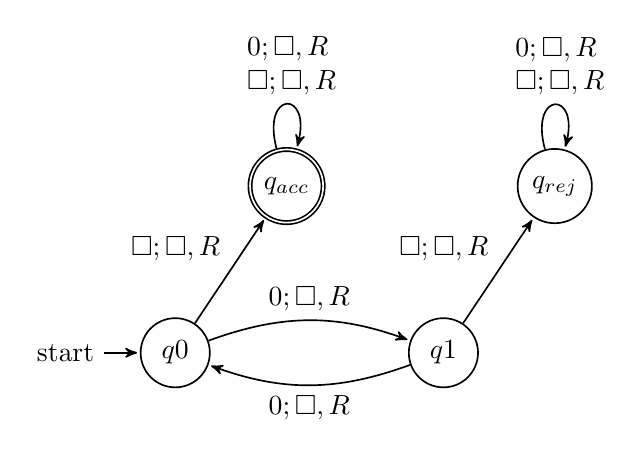
\begin{tikzpicture}[->,>=stealth',shorten >=1pt, auto, node distance=2cm, semithick]
  \tikzstyle{every state}=[text=black, fill=none]
  
  \node[initial,state] (q0)          {$q0$};
  \node[state]         (q1) [right of=q0, xshift=40pt] {$q1$};
  \node[state,accepting]         (qacc) [above right of=q0, yshift=20pt] {$q_{acc}$};
  \node[state]         (qrej) [above right of=q1,yshift=20pt] {$q_{rej}$};
  
  \path (q0) edge [bend left=0] node {$\square; \square, R$} (qacc)
      (q0) edge  [bend left=20] node {$0; \square, R$} (q1)
      (q1) edge [bend left=20] node {$0; \square, R$} (q0)
      (q1) edge [bend left=0] node {$\square; \square, R$} (qrej)
      (qacc) edge  [loop above] node {\parbox{1cm}{$0; \square, R$\newline $\square; \square, R$}} (qacc)
      (qrej) edge  [loop above] node {\parbox{1cm}{$0; \square, R$\newline $\square; \square, R$}}  (qrej)
  ;
\end{tikzpicture}
\columnbreak
Formal definition:

\vspace{10pt}

Sample computation: 

\begin{tabular}{|c|c|c|c|c|c|c|}
\hline
\multicolumn{1}{|c}{$q0\downarrow$} &  \multicolumn{6}{c|}{\phantom{A}}\\
\hline
$0$ & $0$  & $0$ & $\textvisiblespace $& $\textvisiblespace $& $\textvisiblespace $&  $\textvisiblespace $\\
\hline
\multicolumn{7}{|c|}{\phantom{A}}\\
\hline
\phantom{AA} & \phantom{AA}& \phantom{AA}& \phantom{AA}& \phantom{AA}& \phantom{AA}& \phantom{AA} \\
\hline
\multicolumn{7}{|c|}{\phantom{A}}\\
\hline
\phantom{AA} & \phantom{AA}& \phantom{AA}& \phantom{AA}& \phantom{AA}& \phantom{AA}& \phantom{AA} \\
\hline
\multicolumn{7}{|c|}{\phantom{A}}\\
\hline
\phantom{AA} & \phantom{AA}& \phantom{AA}& \phantom{AA}& \phantom{AA}& \phantom{AA}& \phantom{AA} \\
\hline
\multicolumn{7}{|c|}{\phantom{A}}\\
\hline
\phantom{AA} & \phantom{AA}& \phantom{AA}& \phantom{AA}& \phantom{AA}& \phantom{AA}& \phantom{AA} \\
\hline
\end{tabular}
\end{multicols}
\vfill

The language recognized by this machine is \ldots

\vfill
 

{\bf Describing  Turing machines} (Sipser p. 185) To define a Turing machine, we could give a 
\begin{itemize}
\item {\bf Formal definition}: the $7$-tuple of parameters including set of states, 
input alphabet, tape alphabet, transition function, start state, accept state, and reject state; or,
\item {\bf Implementation-level definition}: English prose that describes the Turing machine head 
movements relative to contents of tape, and conditions for accepting / rejecting based on those contents.
\item {\bf High-level description}: description of algorithm (precise sequence of instructions), 
without implementation details of machine. As part of this description, can ``call" and run 
another TM as a subroutine.
\end{itemize}
  
\newpage
Fix $\Sigma = \{0,1\}$, $\Gamma = \{ 0, 1, \textvisiblespace\}$ for the Turing machines with  the following state diagrams:
  
\begin{center}
  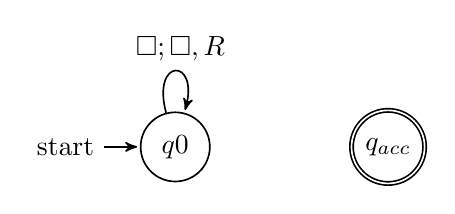
\begin{tikzpicture}[->,>=stealth',shorten >=1pt, auto, node distance=2cm, semithick]
    \tikzstyle{every state}=[text=black, fill=none]
    
    \node[initial,state] (q0)          {$q0$};
    \node[state,accepting]         (qacc) [right of=q0, xshift=20pt] {$q_{acc}$};
    
    \path (q0) edge  [loop above] node {\parbox{1cm}{$\square; \square, R$}} (q0)
    ;
  \end{tikzpicture}
\end{center}

Example of string accepted: \\
Example of string rejected: \\


Implementation-level description

\vfill

High-level description

\vfill

\begin{center}
  \begin{tikzpicture}[->,>=stealth',shorten >=1pt, auto, node distance=2cm, semithick]
    \tikzstyle{every state}=[text=black, fill=none]
    
    \node[initial,state] (qrej)          {$q_{rej}$};
    \node[state,accepting]         (qacc) [right of=q0, xshift=20pt] {$q_{acc}$};
  \end{tikzpicture}
\end{center}

Example of string accepted: \\
Example of string rejected: \\


Implementation-level description

\vfill

High-level description

\vfill

\newpage
\begin{center}
  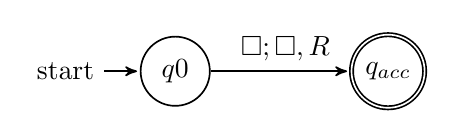
\begin{tikzpicture}[->,>=stealth',shorten >=1pt, auto, node distance=2cm, semithick]
    \tikzstyle{every state}=[text=black, fill=none]
    
    \node[initial,state] (q0)          {$q0$};
    \node[state,accepting]         (qacc) [right of=q0, xshift=20pt] {$q_{acc}$};
    
    \path (q0) edge  [bend left=0] node {\parbox{1cm}{$\square; \square, R$}} (qacc)
    ;
  \end{tikzpicture}
\end{center}

Example of string accepted: \\
Example of string rejected: \\


Implementation-level description

\vfill

High-level description

\vfill

\begin{center}
  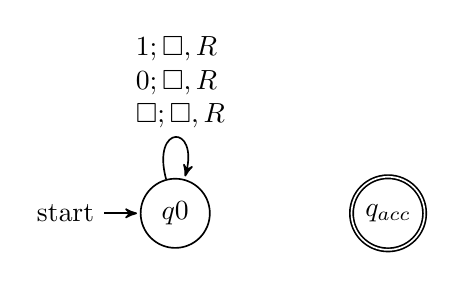
\begin{tikzpicture}[->,>=stealth',shorten >=1pt, auto, node distance=2cm, semithick]
    \tikzstyle{every state}=[text=black, fill=none]
    
    \node[initial,state] (q0)          {$q0$};
    \node[state,accepting]         (qacc) [right of=q0, xshift=20pt] {$q_{acc}$};
    
    \path (q0) edge  [loop above] node {\parbox{1cm}{$1; \square, R$\\$0; \square, R$\\$\square; \square, R$}} (q0)
    ;
  \end{tikzpicture}
\end{center}

Example of string accepted: \\
Example of string rejected: \\


Implementation-level description

\vfill

High-level description

\vfill

\newpage
 \vfill
\section*{Week4 wednesday}



{\bf Definition} A {\bf pushdown automaton} (PDA) is  specified by a  $6$-tuple $(Q, \Sigma, \Gamma, \delta, q_0, F)$
where $Q$ is the finite set of states, $\Sigma$ is the input alphabet,  $\Gamma$ is the stack alphabet,
\[
    \delta: Q \times \Sigma_\varepsilon  \times  \Gamma_\varepsilon \to \mathcal{P}( Q \times \Gamma_\varepsilon)
\]
is the transition function,  $q_0 \in Q$ is the start state, $F \subseteq  Q$ is the set of accept states.


Draw the state diagram and give the formal definition of a PDA with $\Sigma = \Gamma$.

\vfill

Draw the state diagram and give the formal definition of a PDA with $\Sigma \cap \Gamma = \emptyset$.
    
\vfill

\newpage
For the PDA state diagrams below, $\Sigma = \{0,1\}$.


\begin{center}
\begin{tabular}{c c}
Mathematical description of language & State diagram of PDA recognizing language\\
\hline
& $\Gamma = \{ \$, \#\}$ \hspace{2.3in} \\
& \\
& 
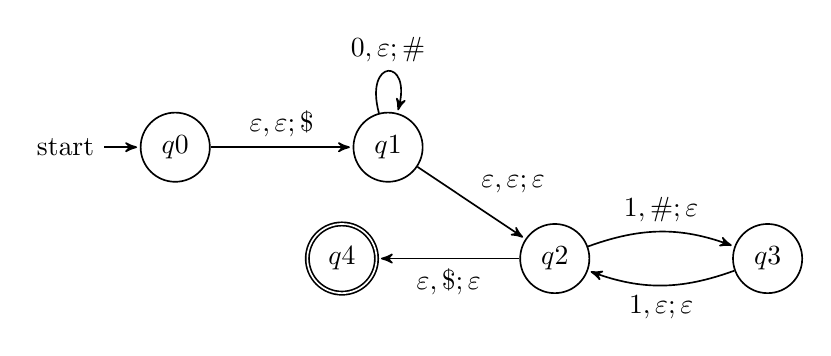
\begin{tikzpicture}[->,>=stealth',shorten >=1pt, auto, node distance=2cm, semithick]
    \tikzstyle{every state}=[text=black, fill=none]
    
    \node[initial,state] (q0)          {$q0$};
    \node[state]         (q1) [right of=q0, xshift=20pt] {$q1$};
    \node[state]         (q2) [below right of=q1, xshift=20pt] {$q2$};
    \node[state]         (q3) [right of=q2, xshift=20pt] {$q3$};
    \node[state,accepting]         (q4) [left of=q2, xshift=-20pt] {$q4$};
    
    \path (q0) edge [bend left=0] node {$\varepsilon, \varepsilon; \$$} (q1)
        (q1) edge  [loop above] node {$0, \varepsilon; \#$} (q1)
        (q1) edge [bend left=0] node {$\varepsilon, \varepsilon; \varepsilon$} (q2)
        (q2) edge  [bend left=20] node [midway, above] {$1, \#; \varepsilon$} (q3)
        (q3) edge  [bend left=20] node [midway, below] {$1, \varepsilon; \varepsilon$} (q2)
        (q2) edge  [bend left=0] node {$\varepsilon, \$; \varepsilon$} (q4)
    ;
\end{tikzpicture}
\\
& \\
& \\
\hline
& $\Gamma = \{ \sun, 1\}$ \hspace{2.3in} \\
& \\
& 
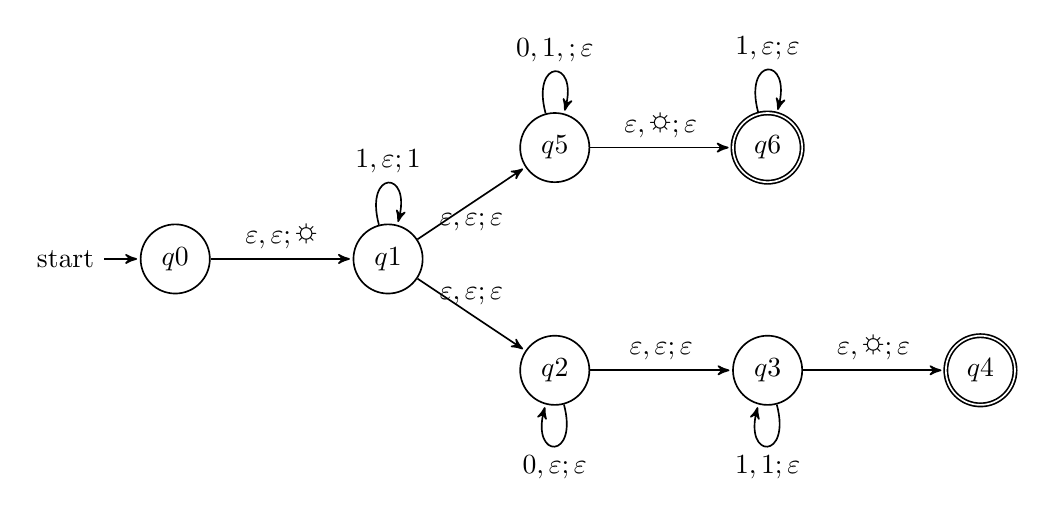
\begin{tikzpicture}[->,>=stealth',shorten >=1pt, auto, node distance=2cm, semithick]
    \tikzstyle{every state}=[text=black, fill=none]
    
    \node[initial,state] (q0)          {$q0$};
    \node[state]         (q1) [right of=q0, xshift=20pt] {$q1$};
    \node[state]         (q2) [below right of=q1, xshift=20pt] {$q2$};
    \node[state]         (q3) [right of=q2, xshift=20pt] {$q3$};
    \node[state,accepting]  (q4) [right of=q3, xshift=20pt] {$q4$};
    \node[state]         (q5) [above right of=q1, xshift=20pt] {$q5$};
    \node[state,accepting]  (q6) [right of=q5, xshift=20pt] {$q6$};
    
    \path (q0) edge [bend left=0] node {$\varepsilon, \varepsilon; \sun$} (q1)
        (q1) edge  [loop above] node {$1, \varepsilon; 1$} (q1)
        (q1) edge [bend left=0] node [below] {$\varepsilon, \varepsilon; \varepsilon$} (q5)
        (q1) edge [bend left=0] node [above]{$\varepsilon, \varepsilon; \varepsilon$} (q2)
        (q5) edge [loop above] node {$0, 1, ; \varepsilon$} (q5)
        (q5) edge [bend left=0] node {$\varepsilon, \sun; \varepsilon$} (q6)
        (q6) edge [loop above] node {$1, \varepsilon; \varepsilon$} (q6)
        (q2) edge [loop below] node {$0, \varepsilon; \varepsilon$} (q2)
        (q2) edge  [bend left=0] node {$\varepsilon, \varepsilon; \varepsilon$} (q3)
        (q3) edge  [loop below] node {$1, 1; \varepsilon$} (q3)
        (q3) edge  [bend left=0] node {$\varepsilon, \sun; \varepsilon$} (q4)
    ;
\end{tikzpicture}
\\
& \\
& \\
\hline
& \\
& \\
& \\
$\{ 0^i 1^j 0^k \mid i,j,k \geq 0 \}$ & \\
& \\
& \\
\end{tabular}
\end{center}

 \vfill
 {\it Note: alternate notation is to replace $;$ with $\to$}

\begin{comment}
{\it Extra practice}: Consider the state diagram of a PDA with input alphabet 
$\Sigma$ and stack alphabet $\Gamma$.

\begin{center}
\begin{tabular}{|c|c|}
\hline
Label & means \\
\hline
$a, b ; c$ when $a \in \Sigma$, $b\in \Gamma$, $c \in \Gamma$ 
& \hspace{3in} \\
& \\
& \\
& \\
& \\
&\\
\hline
$a, \varepsilon ; c$ when $a \in \Sigma$, $c \in \Gamma$ 
& \hspace{3in} \\
& \\
& \\
& \\
& \\
&\\
\hline
$a, b ; \varepsilon$ when $a \in \Sigma$, $b\in \Gamma$
& \hspace{3in} \\
& \\
& \\
& \\
& \\
&\\
\hline
$a, \varepsilon ; \varepsilon$ when $a \in \Sigma$
& \hspace{3in} \\
& \\
& \\
& \\
& \\
&\\
\hline
\end{tabular}
\end{center}


How does the meaning change if $a$ is replaced by $\varepsilon$?
\end{comment}
 \vfill
\section*{Week4 friday}



{\it Big picture}: PDAs were motivated by wanting to add some memory of unbounded size to NFA. How 
do we accomplish a similar enhancement of regular expressions to get a syntactic model that is 
more expressive?

DFA, NFA, PDA: Machines process one input string at a time; the computation of a machine on its input string 
reads the input from left to right.

Regular expressions: Syntactic descriptions of all strings that match a particular pattern; the language 
described by a regular expression is built up recursively according to the expression's syntax

{\bf Context-free grammars}: Rules to produce one string at a time, adding characters from the middle, beginning, 
or end of the final string as the derivation proceeds.\\



Definitions below are on pages 101-102.

\vspace{-20pt}

\begin{center}
    \begin{tabular}{|p{2.4in}cp{3.6in}|}
    \hline 
    {\bf Term} & {\bf Typical symbol} & {\bf Meaning} \\
     & or {\bf Notation} & \\
    \hline
    \hline
    {\bf Context-free grammar} (CFG) & $G$ & $G = (V, \Sigma, R, S)$ \\
    The set of {\bf variables}& $V$ & Finite  set of symbols that represent phases in production pattern\\
    The set of {\bf terminals} & $\Sigma$ & Alphabet of symbols of strings generated  by CFG \\
    & & $V \cap \Sigma = \emptyset$ \\
    The set of {\bf rules}& $R$ & Each rule is  $A \to u$ with $A \in V$ and $u  \in (V  \cup \Sigma)^*$\\
    The {\bf start} variable&  $S$  & Usually  on left-hand-side of first/ topmost rule \\
    & &\\
    {\bf Derivation} & $S \Rightarrow \cdots \Rightarrow w$& 
    Sequence  of substitutions in a  CFG (also written $S \Rightarrow^* w$). At each step, we can apply one rule 
    to one occurrence of a variable in the current string by substituting that occurrence of the variable with the 
    right-hand-side of the rule. The derivation must end when the current string has only terminals (no variables)
    because then there are no instances of variables to apply a rule to.\\
    Language {\bf generated} by the context-free grammar $G$ & $L(G)$ &The set of strings for which there is a derivation in $G$. 
    Symbolically: $\{  w \in \Sigma^* \mid S \Rightarrow^* w \}$ i.e. $$\{  w \in \Sigma^* \mid \text{there is  derivation in $G$ that ends
    in $w$} \}$$\\
    {\bf Context-free language} & & A language that is the language generated by some context-free grammar\\
    \hline
    \end{tabular}
\end{center}

\vfill

\newpage
  
{\bf Examples of context-free grammars, derivations in those grammars, and the languages generated by those grammars}
  
$G_1 =  (\{S\}, \{0\}, R, S)$ with rules
  \begin{align*}
    &S \to 0S\\
    &S \to 0\\
  \end{align*}
  In  $L(G_1)$ \ldots 
  
\vfill

  Not in $L(G_1)$ \ldots 


  \vfill

\newpage
  $G_2 =  (\{S\}, \{0,1\}, R, S)$
  \[
  S \to 0S \mid 1S \mid \varepsilon
  \]
  In  $L(G_2)$ \ldots 
  
  \vspace{110pt}
  
  Not in $L(G_2)$ \ldots 

  \vspace{110pt}

  $(\{S, T\}, \{0, 1\}, R, S)$ with  rules
  \begin{align*}
  &S \to T1T1T1T \\
  &T \to  0T \mid 1T \mid \varepsilon
  \end{align*}

  In  $L(G_3)$ \ldots 
  
  \vspace{110pt}
  
  Not in $L(G_3)$ \ldots 

  \vspace{110pt}

\newpage
  $G_4 =  (\{A, B\}, \{0, 1\}, R, A)$ with rules
  \[
    A \to 0A0 \mid  0A1 \mid 1A0  \mid 1A1 \mid  1
  \]
  In  $L(G_4)$ \ldots 
  
  \vspace{110pt}
  
  Not in $L(G_4)$ \ldots 

  \vspace{110pt}


  \begin{comment}
    I moved the following to the review quiz.

    {\it Extra practice}: Is there a CFG $G$ with $L(G) = \emptyset$?


  Three different CFGs that each generate the  language $\{abba\}$
  
  \begin{align*}
  & ( \{ S, T, V, W\}, \{a,b\}, \{ S \to aT, T \to bV, V \to bW, W \to a\}, S)\\
  & \\ 
  & \\ 
  & \\ 
  & ( \{ Q \}, \{a,b\}, \{Q \to abba\}, Q) \\
  & \\ 
  & \\ 
  & \\
  & ( \{ X,Y \}, \{a,b\}, \{X \to aYa, Y \to bb\}, X) 
  & \\ 
  & \\ 
  \end{align*} 
\end{comment}
  \newpage
  Design a CFG to generate the  language $\{a^n b^n \mid  n  \geq  0\}$
  
  \vspace{100pt}
  
  {\it Sample derivation:} 
  
  \vspace{100pt}
  
  
  \vfill 


\newpage
 \vfill
\section*{Week6 monday}



{\it Sipser Figure  3.10}

{\bf Conventions in state diagram of TM}: $b \to R$ label means $b \to b, R$ and
all arrows missing from diagram represent transitions with output $(q_{reject}, \textvisiblespace , R)$

\begin{multicols}{2}
\vspace{-20pt}
\begin{center}
\includegraphics[width=4in]{../../resources/machines/Lect13TM3.png}
\end{center}

Implementation level description of this machine:
\begin{quote}
Zig-zag across tape to corresponding positions on either side of $\#$ to check whether the 
characters in these positions agree. If they do not, or if there is no $\#$, reject. If they 
do, cross them off.

Once all symbols to the left of the $\#$ are crossed off, check for any un-crossed-off symbols 
to the right of $\#$; if there are any, reject; if there aren't, accept.
\end{quote}

The language recognized by this machine is
\[
  \{ w \# w \mid w \in \{0,1\}^* \}
\]

\columnbreak

Computation on  input  string  $01\#01$

\begin{tabular}{|c|c|c|c|c|c|c|}
\hline
\multicolumn{1}{|c}{$q_1 \downarrow$} &  \multicolumn{6}{c|}{\phantom{A}}\\
\hline
$0$ & $1$  & $\#$  & $0$ & $1$ & $\textvisiblespace $& $\textvisiblespace $\\
\hline
  \multicolumn{7}{|c|}{\phantom{A}}\\
  \hline
  \phantom{AA} & \phantom{AA}& \phantom{AA}& \phantom{AA}& \phantom{AA}& \phantom{AA}& \phantom{AA} \\
  \hline
  \multicolumn{7}{|c|}{\phantom{A}}\\
  \hline
  \phantom{AA} & \phantom{AA}& \phantom{AA}& \phantom{AA}& \phantom{AA}& \phantom{AA}& \phantom{AA} \\
  \hline
  \multicolumn{7}{|c|}{\phantom{A}}\\
  \hline
  \phantom{AA} & \phantom{AA}& \phantom{AA}& \phantom{AA}& \phantom{AA}& \phantom{AA}& \phantom{AA} \\
  \hline
  \multicolumn{7}{|c|}{\phantom{A}}\\
  \hline
  \phantom{AA} & \phantom{AA}& \phantom{AA}& \phantom{AA}& \phantom{AA}& \phantom{AA}& \phantom{AA} \\
  \hline
  \multicolumn{7}{|c|}{\phantom{A}}\\
  \hline
  \phantom{AA} & \phantom{AA}& \phantom{AA}& \phantom{AA}& \phantom{AA}& \phantom{AA}& \phantom{AA} \\
  \hline
  \multicolumn{7}{|c|}{\phantom{A}}\\
  \hline
  \phantom{AA} & \phantom{AA}& \phantom{AA}& \phantom{AA}& \phantom{AA}& \phantom{AA}& \phantom{AA} \\
  \hline
  \multicolumn{7}{|c|}{\phantom{A}}\\
  \hline
  \phantom{AA} & \phantom{AA}& \phantom{AA}& \phantom{AA}& \phantom{AA}& \phantom{AA}& \phantom{AA} \\
  \hline
  \multicolumn{7}{|c|}{\phantom{A}}\\
  \hline
  \phantom{AA} & \phantom{AA}& \phantom{AA}& \phantom{AA}& \phantom{AA}& \phantom{AA}& \phantom{AA} \\
  \hline
  \multicolumn{7}{|c|}{\phantom{A}}\\
  \hline
  \phantom{AA} & \phantom{AA}& \phantom{AA}& \phantom{AA}& \phantom{AA}& \phantom{AA}& \phantom{AA} \\
  \hline
  \multicolumn{7}{|c|}{\phantom{A}}\\
  \hline
  \phantom{AA} & \phantom{AA}& \phantom{AA}& \phantom{AA}& \phantom{AA}& \phantom{AA}& \phantom{AA} \\
  \hline
  \multicolumn{7}{|c|}{\phantom{A}}\\
  \hline
  \phantom{AA} & \phantom{AA}& \phantom{AA}& \phantom{AA}& \phantom{AA}& \phantom{AA}& \phantom{AA} \\
  \hline
  \multicolumn{7}{|c|}{\phantom{A}}\\
  \hline
  \phantom{AA} & \phantom{AA}& \phantom{AA}& \phantom{AA}& \phantom{AA}& \phantom{AA}& \phantom{AA} \\
  \hline
  \multicolumn{7}{|c|}{\phantom{A}}\\
  \hline
  \phantom{AA} & \phantom{AA}& \phantom{AA}& \phantom{AA}& \phantom{AA}& \phantom{AA}& \phantom{AA} \\
  \hline
  \multicolumn{7}{|c|}{\phantom{A}}\\
  \hline
  \phantom{AA} & \phantom{AA}& \phantom{AA}& \phantom{AA}& \phantom{AA}& \phantom{AA}& \phantom{AA} \\
  \hline
  \multicolumn{7}{|c|}{\phantom{A}}\\
  \hline
  \phantom{AA} & \phantom{AA}& \phantom{AA}& \phantom{AA}& \phantom{AA}& \phantom{AA}& \phantom{AA} \\
  \hline
  \multicolumn{7}{|c|}{\phantom{A}}\\
  \hline
  \phantom{AA} & \phantom{AA}& \phantom{AA}& \phantom{AA}& \phantom{AA}& \phantom{AA}& \phantom{AA} \\
  \hline
  \multicolumn{7}{|c|}{\phantom{A}}\\
  \hline
  \phantom{AA} & \phantom{AA}& \phantom{AA}& \phantom{AA}& \phantom{AA}& \phantom{AA}& \phantom{AA} \\
  \hline
  \multicolumn{7}{|c|}{\phantom{A}}\\
  \hline
  \phantom{AA} & \phantom{AA}& \phantom{AA}& \phantom{AA}& \phantom{AA}& \phantom{AA}& \phantom{AA} \\
  \hline
  \end{tabular}
\end{multicols}

\begin{multicols}{2}
High-level description of this machine is

\vfill


{\it Recall:} 
High-level descriptions of  Turing machine algorithms are written as indented text within quotation marks.   
Stages of the algorithm are typically numbered consecutively.
The first line specifies the input to the machine, which must be a string.

\columnbreak

{\it Extra practice}

Computation on  input  string  $01\#1$

\begin{tabular}{|c|c|c|c|c|c|c|}
\hline
\multicolumn{1}{|c}{$q_1\downarrow$} &  \multicolumn{6}{c|}{\phantom{A}}\\
\hline
$0$ & $1$  & $\#$  & $1$ & $\textvisiblespace $& $\textvisiblespace $&  $\textvisiblespace $\\
\hline
\multicolumn{7}{|c|}{\phantom{A}}\\
\hline
\phantom{AA} & \phantom{AA}& \phantom{AA}& \phantom{AA}& \phantom{AA}& \phantom{AA}& \phantom{AA} \\
\hline
\multicolumn{7}{|c|}{\phantom{A}}\\
\hline
\phantom{AA} & \phantom{AA}& \phantom{AA}& \phantom{AA}& \phantom{AA}& \phantom{AA}& \phantom{AA} \\
\hline
\multicolumn{7}{|c|}{\phantom{A}}\\
\hline
\phantom{AA} & \phantom{AA}& \phantom{AA}& \phantom{AA}& \phantom{AA}& \phantom{AA}& \phantom{AA} \\
\hline
\multicolumn{7}{|c|}{\phantom{A}}\\
\hline
\phantom{AA} & \phantom{AA}& \phantom{AA}& \phantom{AA}& \phantom{AA}& \phantom{AA}& \phantom{AA} \\
\hline
\multicolumn{7}{|c|}{\phantom{A}}\\
\hline
\phantom{AA} & \phantom{AA}& \phantom{AA}& \phantom{AA}& \phantom{AA}& \phantom{AA}& \phantom{AA} \\
\hline
\multicolumn{7}{|c|}{\phantom{A}}\\
\hline
\phantom{AA} & \phantom{AA}& \phantom{AA}& \phantom{AA}& \phantom{AA}& \phantom{AA}& \phantom{AA} \\
\hline
\multicolumn{7}{|c|}{\phantom{A}}\\
\hline
\phantom{AA} & \phantom{AA}& \phantom{AA}& \phantom{AA}& \phantom{AA}& \phantom{AA}& \phantom{AA} \\
\hline
\multicolumn{7}{|c|}{\phantom{A}}\\
\hline
\phantom{AA} & \phantom{AA}& \phantom{AA}& \phantom{AA}& \phantom{AA}& \phantom{AA}& \phantom{AA} \\
\hline
\multicolumn{7}{|c|}{\phantom{A}}\\
\hline
\phantom{AA} & \phantom{AA}& \phantom{AA}& \phantom{AA}& \phantom{AA}& \phantom{AA}& \phantom{AA} \\
\hline
\multicolumn{7}{|c|}{\phantom{A}}\\
\hline
\phantom{AA} & \phantom{AA}& \phantom{AA}& \phantom{AA}& \phantom{AA}& \phantom{AA}& \phantom{AA} \\
\hline
\multicolumn{7}{|c|}{\phantom{A}}\\
\hline
\phantom{AA} & \phantom{AA}& \phantom{AA}& \phantom{AA}& \phantom{AA}& \phantom{AA}& \phantom{AA} \\
\hline
\multicolumn{7}{|c|}{\phantom{A}}\\
\hline
\phantom{AA} & \phantom{AA}& \phantom{AA}& \phantom{AA}& \phantom{AA}& \phantom{AA}& \phantom{AA} \\
\hline
\multicolumn{7}{|c|}{\phantom{A}}\\
\hline
\phantom{AA} & \phantom{AA}& \phantom{AA}& \phantom{AA}& \phantom{AA}& \phantom{AA}& \phantom{AA} \\
\hline
\multicolumn{7}{|c|}{\phantom{A}}\\
\hline
\phantom{AA} & \phantom{AA}& \phantom{AA}& \phantom{AA}& \phantom{AA}& \phantom{AA}& \phantom{AA} \\
\hline
\multicolumn{7}{|c|}{\phantom{A}}\\
\hline
\phantom{AA} & \phantom{AA}& \phantom{AA}& \phantom{AA}& \phantom{AA}& \phantom{AA}& \phantom{AA} \\
\hline
\multicolumn{7}{|c|}{\phantom{A}}\\
\hline
\phantom{AA} & \phantom{AA}& \phantom{AA}& \phantom{AA}& \phantom{AA}& \phantom{AA}& \phantom{AA} \\
\hline
\multicolumn{7}{|c|}{\phantom{A}}\\
\hline
\phantom{AA} & \phantom{AA}& \phantom{AA}& \phantom{AA}& \phantom{AA}& \phantom{AA}& \phantom{AA} \\
\hline
\multicolumn{7}{|c|}{\phantom{A}}\\
\hline
\phantom{AA} & \phantom{AA}& \phantom{AA}& \phantom{AA}& \phantom{AA}& \phantom{AA}& \phantom{AA} \\
\hline
\multicolumn{7}{|c|}{\phantom{A}}\\
\hline
\phantom{AA} & \phantom{AA}& \phantom{AA}& \phantom{AA}& \phantom{AA}& \phantom{AA}& \phantom{AA} \\
\hline
\multicolumn{7}{|c|}{\phantom{A}}\\
\hline
\phantom{AA} & \phantom{AA}& \phantom{AA}& \phantom{AA}& \phantom{AA}& \phantom{AA}& \phantom{AA} \\
\hline
\end{tabular}

\end{multicols}
\newpage



A language $L$ is {\bf recognized by} a Turing machine $M$ means

\vfill

A Turing  machine  $M$ {\bf  recognizes} a language $L$ means

\vfill

A Turing machine $M$ is a {\bf decider}  means

\vfill

A language  $L$ is {\bf decided by} a Turing  machine  $M$  means

\vfill

A  Turing machine $M$ {\bf decides} a language $L$ means

\vfill

Fix $\Sigma = \{0,1\}$, $\Gamma = \{ 0, 1, \textvisiblespace\}$ for the Turing machines with  the following state diagrams:
  
  \begin{center}
  \begin{tabular}{|c|c|}
  \hline
  \hspace{0.8in}
  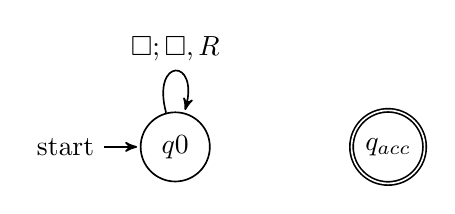
\begin{tikzpicture}[->,>=stealth',shorten >=1pt, auto, node distance=2cm, semithick]
    \tikzstyle{every state}=[text=black, fill=none]
    
    \node[initial,state] (q0)          {$q0$};
    \node[state,accepting]         (qacc) [right of=q0, xshift=20pt] {$q_{acc}$};
    
    \path (q0) edge  [loop above] node {$\square; \square, R$} (qacc)
    ;
  \end{tikzpicture}
\phantom{\hspace{0.8in}}&\hspace{0.8in} 
  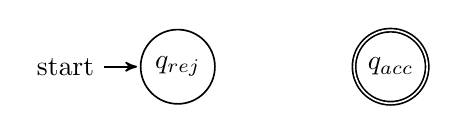
\begin{tikzpicture}[->,>=stealth',shorten >=1pt, auto, node distance=2cm, semithick]
    \tikzstyle{every state}=[text=black, fill=none]
    
    \node[initial,state] (qrej)          {$q_{rej}$};
    \node[state,accepting]         (qacc) [right of=qrej, xshift=20pt] {$q_{acc}$};
  \end{tikzpicture}
  \phantom{\hspace{0.8in}}\\
  Decider? Yes~~~/ ~~~No
  &Decider? Yes~~~/ ~~~No\\
  & \\
  \hline

  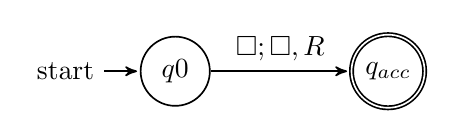
\begin{tikzpicture}[->,>=stealth',shorten >=1pt, auto, node distance=2cm, semithick]
    \tikzstyle{every state}=[text=black, fill=none]
    
    \node[initial,state] (q0)          {$q0$};
    \node[state,accepting]         (qacc) [right of=q0, xshift=20pt] {$q_{acc}$};

    \path (q0) edge [bend left=0] node {$\square; \square, R$} (qacc)
    ;
  \end{tikzpicture} & 
  
  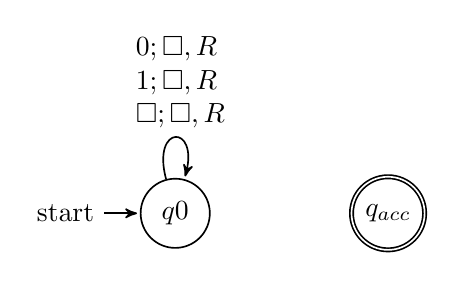
\begin{tikzpicture}[->,>=stealth',shorten >=1pt, auto, node distance=2cm, semithick]
    \tikzstyle{every state}=[text=black, fill=none]
    
    \node[initial,state] (q0)          {$q0$};
    \node[state,accepting]         (qacc) [right of=q0, xshift=20pt] {$q_{acc}$};
    
    \path (q0) edge  [loop above] node {\parbox{1cm}{$0; \square, R$\newline$1; \square, R$\newline $\square; \square, R$}} (q0)
    ;
  \end{tikzpicture}\\
  Decider? Yes~~~/ ~~~No
  &Decider? Yes~~~/ ~~~No\\
  & \\
  
  \hline
  \end{tabular}
  \end{center}
  \newpage

 \vfill
\section*{Week6 wednesday}




A {\bf Turing-recognizable} language is a set of strings that 
is the language recognized by some Turing machine. We also 
say that such languages are recognizable.

A {\bf Turing-decidable} language is a set of strings that 
is the language recognized by some decider. We also 
say that such languages are decidable.


An {\bf unrecognizable} language is a language that is not Turing-recognizable.

An {\bf undecidable} language is a language that is not Turing-decidable.

\vfill

{\bf  True} or {\bf False}: Any  decidable language  is  also  recognizable.

\vfill

{\bf  True} or {\bf False}: Any  recognizable language  is  also  decidable.

\vfill

{\bf  True} or {\bf False}: Any  undecidable language  is  also  unrecognizable.

\vfill

{\bf  True} or {\bf False}: Any  unrecognizable language  is  also  undecidable.

\vfill

\newpage


{\bf True} or {\bf False}: The class of Turing-decidable languages is closed under complementation.

\vfill

Using formal definition:
\vfill

Using high-level description:
\vfill


{\bf  Church-Turing Thesis} (Sipser p. 183): The informal notion of algorithm is formalized completely  and correctly by the 
formal definition of a  Turing machine. In other words: all reasonably expressive models of 
computation are equally expressive with the standard Turing machine.
 \vfill
\section*{Week6 friday}



Definition: A language $L$ over an  alphabet $\Sigma$ is called {\bf co-recognizable} if its complement,  defined
as $\Sigma^* \setminus L  = \{ x  \in  \Sigma^* \mid x \notin  L \}$, is Turing-recognizable.


\vfill 
{\bf  Theorem} (Sipser Theorem 4.22): A  language is Turing-decidable if and only if both  it and its complement
are Turing-recognizable.

{\bf Proof, first direction:}  Suppose  language  $L$ is  Turing-decidable.   WTS  that both it and its complement 
are Turing-recognizable.

\vfill

{\bf Proof, second direction:}  Suppose  language  $L$ is  Turing-recognizable, and  so is  its complement.   WTS  that $L$
is Turing-decidable.
\vfill


Notation: The complement  of a set $X$ is denoted with  a superscript $c$, $X^c$, or an overline,  $\overline{X}$.

\newpage

{\bf Claim}: If two languages  (over a fixed alphabet  $\Sigma$) are Turing-decidable, then  their union  is  as well.

{\bf Proof}:


\vfill
\newpage

{\bf Claim}: If two languages  (over a fixed alphabet  $\Sigma$) are Turing-recognizable, then  their union  is  as well.

{\bf Proof}:

 \vfill
\section*{Week7 wednesday}


{\bf The Church-Turing thesis posits that each algorithm can be implemented by some Turing machine.}

{\bf Describing  algorithms} (Sipser p. 185) To define a Turing machine, we could give a 
\begin{itemize}
\item {\bf Formal definition}: the $7$-tuple of parameters including set of states, 
input alphabet, tape alphabet, transition function, start state, accept state, and reject state.
This is the low-level programming view that models the logic computation flow in a processor.
\item {\bf Implementation-level definition}: English prose that describes the Turing machine head 
movements relative to contents of tape, and conditions for accepting / rejecting based on those contents.
This level describes memory management and implementing data access with data structures.
  \begin{itemize}
    \item Mention the tape or its contents (e.g.\ ``Scan the tape from left to right until a blank is seen.'')
    \item Mention the tape head (e.g.\ ``Return the tape head to the left end of the tape.'')
  \end{itemize}
\item {\bf High-level description} of algorithm executed by Turing machine: 
description of algorithm (precise sequence of instructions), 
without implementation details of machine. 
High-level descriptions of  Turing machine algorithms are written as indented text within quotation marks.   
Stages of the algorithm are typically numbered consecutively.
The first line specifies the input to the machine, which must be a string.
  \begin{itemize}
    \item Use other Turing machines as subroutines (e.g.\ ``Run $M$ on $w$'')
    \item Build new machines from existing machines using previously shown results (e.g.\ 
    ``Given NFA $A$ construct an NFA $B$ such that $L(B) = \overline{L(A)}$'')
    \item Use previously shown conversions and constructions (e.g.\ ``Convert regular expression $R$ 
    to an NFA $N$'')
  \end{itemize}
\end{itemize}

{\bf Formatted inputs to Turing machine algorithms}

The input to a Turing machine is always a string. 
The format of the input to a Turing machine can be checked to interpret 
this string as representing structured data (like a csv file, the formal definition of a DFA, another Turing machine, etc.)


This string may be the encoding of some object or  list of  objects.  

{\bf Notation:} $\langle O \rangle$ is the string that encodes the object $O$.
$\langle O_1, \ldots, O_n \rangle$ is the string that encodes the list of objects $O_1, \ldots, O_n$.

{\bf Assumption}: There are algorithms (Turing  machines) that can be called as subroutines
to decode the string representations of common objects and  interact with these objects as intended
(data structures). These algorithms are able to ``type-check'' and string representations for different
data structures are unique.
  
\newpage
For example, since there are algorithms to answer each of the following questions,
by Church-Turing thesis, there is a Turing machine that accepts exactly those strings for which the 
answer to the question is ``yes''
\begin{itemize}
    \item Does a string over $\{0,1\}$ have even length?

    \item Does a string over $\{0,1\}$ encode a string of ASCII characters?\footnote{An introduction to ASCII 
    is available on the w3 tutorial \href{https://www.w3schools.com/charsets/ref_html_ascii.asp}{here}.}

    \item Does a DFA have a specific number of states?

    \item Do two NFAs have any state names in common?

    \item Do two CFGs have the same start variable?

  \end{itemize}



A {\bf computational problem} is decidable iff language encoding its positive problem instances
is decidable.

The computational problem ``Does a specific DFA accept a given string?'' is encoded by the language
\begin{align*}
  &\{ \textrm{representations of DFAs $M$ and strings $w$ such that $w \in L(M)$}\}  \\
  =& \{ \langle M, w \rangle \mid M \textrm{ is a DFA}, w \textrm{ is a string}, w \in L(M) \}
\end{align*}

The computational problem ``Is the language generated by a CFG empty?'' is encoded by the language
\begin{align*}
  &\{ \textrm{representations of CFGs $G$  such that $L(G) = \emptyset$}\}  \\
  =& \{ \langle G \rangle \mid G \textrm{ is a CFG},  L(G) = \emptyset \}
\end{align*}



The computational problem ``Is the given Turing machine a decider?'' is encoded by the language
\begin{align*}
  &\{ \textrm{representations of TMs $M$  such that $M$ halts on every input}\}  \\
  =& \{ \langle M \rangle \mid M \textrm{ is a TM and for each string } w, \textrm{$M$ halts on $w$} \}
\end{align*}


{\it Note: writing down the language encoding a computational problem is only the first step in 
determining if it's recognizable, decidable, or \ldots }

Deciding a computational problem means building / defining a Turing 
machine that recognizes the language encoding the computational problem, and that 
is a decider.


Some classes of computational problems will 
help us understand the differences between the machine models we've been studying. (Sipser Section 4.1)

    \begin{center}
    \begin{tabular}{|lcl|}
    \hline
    \multicolumn{3}{|l|}{{\bf  Acceptance problem} } \\
    & & \\
    \ldots for DFA & $A_{DFA}$ & $\{ \langle B,w \rangle \mid  \text{$B$ is a  DFA that accepts input 
    string $w$}\}$ \\
    \ldots for NFA & $A_{NFA}$ & $\{ \langle B,w \rangle \mid  \text{$B$ is a  NFA that accepts input 
    string $w$}\}$ \\
    \ldots for regular expressions & $A_{REX}$ & $\{ \langle R,w \rangle \mid  \text{$R$ is a  regular
    expression that generates input string $w$}\}$ \\
    \ldots for CFG & $A_{CFG}$ & $\{ \langle G,w \rangle \mid  \text{$G$ is a context-free grammar 
    that generates input string $w$}\}$ \\
    \ldots for PDA & $A_{PDA}$ & $\{ \langle B,w \rangle \mid  \text{$B$ is a PDA that accepts input string $w$}\}$ \\
    & & \\
    \hline
    \multicolumn{3}{|l|}{{\bf Language emptiness  testing} } \\
    & & \\
    \ldots for DFA & $E_{DFA}$ & $\{ \langle A \rangle \mid  \text{$A$ is a  DFA and  $L(A) = \emptyset$\}}$ \\
    \ldots for NFA & $E_{NFA}$ & $\{ \langle A\rangle \mid  \text{$A$ is a NFA and  $L(A) = \emptyset$\}}$ \\
    \ldots for regular expressions & $E_{REX}$ & $\{ \langle R \rangle \mid  \text{$R$ is a  regular
    expression and  $L(R) = \emptyset$\}}$ \\
    \ldots for CFG & $E_{CFG}$ & $\{ \langle G \rangle \mid  \text{$G$ is a context-free grammar 
    and  $L(G) = \emptyset$\}}$ \\
    \ldots for PDA & $E_{PDA}$ & $\{ \langle A \rangle \mid  \text{$A$ is a PDA and  $L(A) = \emptyset$\}}$ \\
    & & \\
    \hline
    \multicolumn{3}{|l|}{{\bf Language equality testing} } \\
    & & \\
    \ldots for DFA & $EQ_{DFA}$ & $\{ \langle A, B \rangle \mid  \text{$A$ and $B$ are DFAs and  $L(A) =L(B)$\}}$\\
    \ldots for NFA & $EQ_{NFA}$ & $\{ \langle A, B \rangle \mid  \text{$A$ and $B$ are NFAs and  $L(A) =L(B)$\}}$\\
    \ldots for regular expressions & $EQ_{REX}$ & $\{ \langle R, R' \rangle \mid  \text{$R$ and $R'$ are regular
    expressions and  $L(R) =L(R')$\}}$\\
    \ldots for CFG & $EQ_{CFG}$ & $\{ \langle G, G' \rangle \mid  \text{$G$ and $G'$ are CFGs and  $L(G) =L(G')$\}}$ \\
    \ldots for PDA & $EQ_{PDA}$ & $\{ \langle A, B \rangle \mid  \text{$A$ and $B$ are PDAs and  $L(A) =L(B)$\}}$ \\
    \hline
    \end{tabular}
    \end{center}
    

    Example strings in $A_{DFA}$
    
    \vfill
    
    Example strings in  $E_{DFA}$
    
    \vfill
    
    Example strings in  $EQ_{DFA}$
    
    \vfill
 \vfill
\section*{Week7 friday}


  \begin{quote}
  $M_1 = $ ``On input $\langle M,w\rangle$, where $M$ is a DFA and $w$ is a string:
  \begin{enumerate}
  \setcounter{enumi}{-1}
  \item Type check encoding to check input is correct type. If not, reject.
  \item Simulate $M$ on input $w$ (by keeping track of states in $M$, transition function of $M$, etc.) 
  \item If the simulations ends in an accept state of $M$, accept. If it ends in a non-accept state of $M$, reject. "
  \end{enumerate}
  \end{quote}
  

What is $L(M_1)$? 

\vfill

Is $M_1$ a decider?

\vfill


{\it Alternate description}:
Sometimes omit step 0 from listing and do implicit type check.

Synonyms: ``Simulate'', ``run'', ``call''.

\newpage

  True / False: $A_{REX} = A_{NFA} = A_{DFA}$

  True / False: $A_{REX} \cap A_{NFA} = \emptyset$, $A_{REX} \cap A_{DFA} = \emptyset$, $A_{DFA} \cap A_{NFA} = \emptyset$

  
  A Turing machine that  decides $A_{NFA}$ is: 
  
  \vfill
  
  A Turing machine that  decides $A_{REX}$ is: 
  
  \vfill

  $E_{DFA} = \{ \langle A \rangle \mid  \text{$A$ is a  DFA and  $L(A) = \emptyset$}\}$. 
  True/False: A Turing machine that  decides $E_{DFA}$ is

  \begin{quote}
  $M_2 =  $``On  input  $\langle M\rangle$ where $M$ is a  DFA,
  \begin{enumerate}
  \item For integer  $i = 1, 2, \ldots$
  \item \qquad Let  $s_i$ be the  $i$th string over  the alphabet of  $M$ (ordered in  string order).
  \item \qquad Run $M$ on  input  $s_i$.
  \item \qquad If $M$  accepts,  $\underline{\phantom{FILL  IN BLANK}}$.  If $M$  rejects, increment $i$ and keep going."
  \end{enumerate}
  \end{quote}
  

Choose the correct option to help fill in the blank so that $M_2$ recognizes $E_{DFA}$
\begin{itemize}
\item[A.] accepts
\item[B.] rejects
\item[C.] loop for ever
\item[D.] We can't fill in the blank in any way to make this work
\end{itemize}

\newpage
  

  
  \begin{quote}
  $M_3 =  $ `` On  input $\langle M \rangle$ where $M$ is  a  DFA,
  \begin{enumerate}
  \item Mark the start  state  of $M$.
  \item Repeat until no  new states get marked:
  \item \qquad Loop over the states of $M$. 
  \item \qquad Mark any unmarked  state  that  has an incoming  edge  from a marked state.
  \item If  no  accept state of $A$ is  marked, $\underline{\phantom{FILL  IN BLANK}}$;  otherwise, 
  $\underline{\phantom{FILL  IN BLANK}}$".
  \end{enumerate}
  \end{quote}
  
  
  
To build a Turing machine that decides $EQ_{DFA}$, notice that 
\[
L_1 = L_2 \qquad\textrm{iff}\qquad (~(L_1 \cap \overline{L_2}) \cup (L_2 \cap \overline L_1)~) = \emptyset  
\]
{\it There are no elements that are in one set and not the other}


$M_{EQDFA} = $ 


  \vfill
  

  {\bf Summary}:  We can use the decision procedures (Turing machines) of decidable problems
  as subroutines in other algorithms. For example, we have subroutines for deciding each of 
  $A_{DFA}$, $E_{DFA}$, $EQ_{DFA}$.  We can also use algorithms for known constructions
  as subroutines in other algorithms. For example, we have subroutines for: counting the number 
  of states in a state diagram, counting the number of characters in an alphabet, converting DFA
  to a DFA recognizing the complement of the original language or a DFA recognizing the 
  Kleene star of the original language, constructing a DFA or NFA from two DFA or NFA so that 
  we have a machine recognizing the language of the union (or intersection, concatenation)
  of the languages of the original machines; converting regular expressions to equivalent DFA; 
  converting DFA to equivalent regular expressions, etc.
 \vfill
\section*{Week3 wednesday}


{\bf Definition and Theorem}: For an alphabet $\Sigma$, a language $L$ over $\Sigma$ is called {\bf regular}
exactly when $L$ is recognized by some DFA, which happens exactly when $L$ is recognized by some NFA, 
and happens exactly when $L$ is described by some regular expression

{\bf We saw that}: The class of regular languages is closed under complementation, union, 
intersection, set-wise concatenation, and Kleene star.

{\bf Prove or Disprove}: There is some alphabet $\Sigma$ for which there is 
some language recognized by an NFA but not by any DFA.

\vfill

{\bf Prove or Disprove}: There is some alphabet $\Sigma$ for which there is 
some finite language not described by any regular expression over $\Sigma$.

\vfill

{\bf Prove or Disprove}: If a language is recognized by an NFA 
then the complement of this language is not recognized by any DFA.

\vfill

\newpage

{\bf Fix alphabet $\Sigma$. Is every language $L$ over $\Sigma$ regular?}

\begin{center}
\begin{tabular}{c|c}
Set & Cardinality \\
\hline
& \\
$\{0,1\}$ & \\
& \\
$\{0,1\}^*$ & \\
& \\
$\mathcal{P}( \{0,1\})$ & \\
& \\
The set of all languages over $\{0,1\}$ & \\
& \\
The set of all regular expressions over $\{0,1\}$ & \\
& \\
The set of all regular languages over $\{0,1\}$ & \\
& \\
\end{tabular}
\end{center}



\vfill
Strategy: Find an {\bf invariant} property that is true of all regular languages. When analyzing 
a given language, if the invariant is not true about it, then the language is not regular.
\newpage

{\bf Pumping Lemma} (Sipser Theorem 1.70): If $A$ is a regular language, then there
is a number $p$ (a {\it pumping length}) where, if $s$ is any string in $A$ of length at least $p$, 
then $s$ may be divided into three pieces, $s = xyz$ such that
\vspace{-10pt}
\begin{itemize}
\item $|y| > 0$
\item for each $i \geq 0$, $xy^i z \in A$
\item $|xy| \leq p$.
\end{itemize}


{\bf Proof illustration}


\vfill




{\bf True or False}: A pumping length for $A = \{ 0,1 \}^*$ is $p = 5$.

\vfill \vfill
\section*{Week3 friday}


Recap so far: In DFA, the only memory available is in the states. Automata can only
``remember'' finitely far in the past and finitely much information, because
they can have only finitely many states. If a computation path of a DFA visits 
the same state more than once, the machine can't tell the difference between 
the first time and future times it visits this state. Thus, if 
a DFA accepts one long string, then it must accept (infinitely) many 
similar strings.

{\bf Definition}  A positive integer $p$ is a {\bf pumping length} of a language $L$ over $\Sigma$ means
that, for each string $s  \in  \Sigma^*$, if  $|s| \geq p$ and $s \in L$, then there are strings $x,y,z$
such that 
\[
s = xyz
\]
and  
\[
|y| > 0,  \qquad \qquad 
\text{ for each $i \geq 0$, $xy^i z \in L$}, \qquad \text{and}
\qquad  \qquad
|xy| \leq p.
\]

{\bf Negation}: A positive integer  $p$  is {\bf not a pumping length} of a language  $L$ over  $\Sigma$  iff
\[
\exists s \left(~  |s| \geq  p \wedge s \in L \wedge \forall x \forall y \forall z  \left( ~\left( s = xyz \wedge 
|y| > 0 \wedge |xy| \leq p~ \right) \to \exists i  (  i \geq 0  \wedge xy^iz  \notin L ) \right) ~\right) 
\]
{\it Informally: }


Restating {\bf Pumping Lemma}: If $L$ is a regular language, then it  has
a pumping length.


{\bf Contrapositive}: If $L$ has no pumping length, then  it is nonregular.

\vfill

{\Large The Pumping Lemma {\it cannot} be used to prove that a language {\it is} regular.} 

{\Large The Pumping Lemma {\bf can} be used to prove that a language {\it is not} regular.}

{\it Extra practice}: Exercise 1.49 in the book.


\vfill

{\bf Proof strategy}: To prove that a language $L$ is {\bf not} regular, 
\begin{itemize}
    \item Consider an arbitrary positive integer $p$
    \item Prove that $p$ is not a pumping length for $L$
    \item Conclude that $L$ does not have {\it any} pumping length, and therefore it is not regular.
\end{itemize}

\newpage
{\bf Example}: $\Sigma  =  \{0,1\}$, $L = \{ 0^n 1^n \mid n  \geq 0\}$.

Fix $p$ an arbitrary positive integer. List strings that are in $L$ and have length  greater than or equal  to $p$:

\vspace{20pt}

Pick $s = $


Suppose $s = xyz$ with  $|xy|  \leq  p$ and $|y| > 0$.
\begin{center}
\begin{tabular}{|c|}
\hline
 \\
\hspace{4in} \\
\hline
\end{tabular}
\end{center}

Then when $i = \hspace{1in}$, $xy^i z  = \hspace{1in}$

\newpage

{\bf Example}: $\Sigma  =  \{0,1\}$, $L = \{w w^{\mathcal{R}} \mid w \in \{0,1\}^*\}$.
Remember that the reverse of a string $w$ is denoted $w^\mathcal{R}$  
and means to write $w$  in  the opposite order, if $w = w_1 \cdots  w_n$ then $w^\mathcal{R} = w_n \cdots  w_1$. Note: $\varepsilon^\mathcal{R} = \varepsilon$.


Fix $p$ an arbitrary positive integer. List strings that are in $L$ and have length  greater than or equal  to $p$:

\vspace{10pt}

Pick $s = $

Suppose $s = xyz$ with  $|xy|  \leq  p$ and $|y| > 0$.
\begin{center}
\begin{tabular}{|c|}
\hline
 \\
\hspace{4in} \\
\hline
\end{tabular}
\end{center}
Then when $i = \hspace{1in}$, $xy^i z  = \hspace{1in}$


\vspace{30pt} 

{\bf Example}: $\Sigma  =  \{0,1\}$, $L = \{0^j1^k  \mid j \geq k  \geq 0\}$.

Fix $p$ an arbitrary positive integer. List strings that are in $L$ and have length  greater than or equal  to $p$:

\vspace{10pt}

Pick $s = $


Suppose $s = xyz$ with  $|xy|  \leq  p$ and $|y| > 0$.
\begin{center}
\begin{tabular}{|c|}
\hline
 \\
\hspace{4in} \\
\hline
\end{tabular}
\end{center}
Then when $i = \hspace{1in}$, $xy^i z  = \hspace{1in}$



\vspace{30pt} 

{\bf Example}: $\Sigma  =  \{0,1\}$, $L = \{0^n1^m0^n  \mid m,n  \geq 0\}$.

Fix $p$ an arbitrary positive integer. List strings that are in $L$ and have length  greater than or equal  to $p$:

\vspace{10pt}

Pick $s = $


Suppose $s = xyz$ with  $|xy|  \leq  p$ and $|y| > 0$.
\begin{center}
\begin{tabular}{|c|}
\hline
 \\
\hspace{4in} \\
\hline
\end{tabular}
\end{center}
Then when $i = \hspace{1in}$, $xy^i z  = \hspace{1in}$

\newpage
{\it Extra practice}:


\begin{center}
    \begin{tabular}{c|c| c| c}
    Language & $s \in L$ & $s \notin L$ & Is the language regular or nonregular?  \\
    \hline
     & \hspace{1in} & \hspace{1in}  &  \\
    $\{a^nb^n \mid 0  \leq n  \leq 5 \}$ & & & \\
     & & & \\
    $\{b^n a^n \mid  n  \geq 2\}$  & & & \\
     & & & \\
    $\{a^m b^n \mid  0 \leq m\leq n\}$  & & & \\
     & & & \\
    $\{a^m b^n \mid  m \geq n+3,  n \geq 0\}$  & & & \\
     & & & \\
    $\{b^m a^n \mid  m \geq 1, n \geq  3\}$  & & & \\
     & & & \\
    $\{ w  \in \{a,b\}^* \mid w = w^\mathcal{R} \}$ & & & \\
     & & & \\ 
    $\{ ww^\mathcal{R} \mid w\in \{a,b\}^* \}$ & & & \\
     & & & \\ 
    \end{tabular}
\end{center}
     \vfill
\end{document}